\begin{task}
\TT{Wyznacz współczynniki trygonometrycznego szeregu Fouriera dla okresowego sygnału $f(t)$ przedstawionego na rysunku}{Calculate coefficients of the periodic signal $f(t)$ shown below for the expansion into a trigonometric Fourier series.} 

\begin{figure}[H]
\centering
\begin{tikzpicture}
  %\draw (0,0) circle (1in);
  \draw[->] (-3.0,+0.0) -- (+5.0,+0.0) node[right] {$t$};
  \draw[->] (+0.0,-1.5) -- (+0.0,+1.5) node[above] {$f(t)$};
  \draw[-,red, thick] (-2.5,+0.0) -- (-2.0,+0.0) -- (-2.0,+1.0) -- (-1.0,+1.0) -- (-1.0,+0.0)--(+0.0,+0.0) -- (+0.0,+1.0) -- (+1.0,+1.0) -- (+1.0,+0.0) -- (+2.0,+0.0) -- (+2.0,+1.0) -- (3.0,1.0) -- (3.0,0.0) -- (3.5,0.0);
  %\draw[-] (-1.0-0.1,-0.1)--(-1.0+0.1,0.1) node[midway, below, outer sep=10pt,align=center] {$-\frac{T}{2}$};
  \draw[-] (-1.0-0.1,-0.1)--(-1.0+0.1,0.1) node[midway, below, outer sep=5pt,align=center] {$-\frac{T}{2}$};
  \draw[-] (+1.0-0.1,-0.1)--(+1.0+0.1,0.1) node[midway, below, outer sep=5pt] {$\frac{T}{2}$};
  \draw[-] (+2.0-0.1,-0.1)--(+2.0+0.1,0.1) node[midway, below, outer sep=5pt] {$T$};
  \draw[-] (-0.1,1.0-0.1)--(+0.1,1.0+0.1) node[midway, left] {$A$};
\end{tikzpicture}
\end{figure}

\TT{W pierwszej kolejności należy opisać sygnał za pomocą wzoru.}{Periodic signal $f(t)$, as a piecewise linear function, is given by:}

\begin{equation}
   f(x)=\begin{cases}A & t \in \left (  0+k \cdot T; \frac{T}{2}+k \cdot T \right ) \\0 & t \in \left ( \frac{T}{2}+k \cdot T; T +k \cdot T\right )\end{cases} \wedge k \in \TT{C}{Z}
\end{equation}

\TT{Współczynnik $a_0$ wyznaczamy ze wzoru:}{The $a_0$ coefficient is defined as:}

\begin{equation}
a_0=\frac{1}{T}\int_{T}f(t) \cdot dt
\end{equation}

\TT{Podstawiamy do wzoru wzór naszej funkcji w pierwszym okresie $k=0$}{For the period $t \in (0; T)$, e.g. $k=0$, we get:}

\begin{equation}
\begin{aligned}
a_0 &=\frac{1}{T}\int_{T}f(t) \cdot dt =\\
&=\frac{1}{T} \left( \int_{0}^{\frac{T}{2}} A \cdot dt + \int_{\frac{T}{2}}^{T} 0 \cdot dt \right ) = \\
&=\frac{1}{T} \left( A \cdot \int_{0}^{\frac{T}{2}} dt + 0 \right ) = \\
&=\frac{1}{T} \left( A \cdot \left. t\right |_{0}^{\frac{T}{2}} \right ) = \\
&=\frac{A}{T} \cdot \left. t\right |_{0}^{\frac{T}{2}} = \\
&=\frac{A}{T} \cdot \left( \frac{T}{2} - 0 \right ) = \\
&=\frac{A}{T} \cdot \left( \frac{T}{2} \right ) = \\
&=\frac{A}{2} 
\end{aligned}
\end{equation}

\TT{Wartość współczynnika $a_0$ wynosi $\frac{A}{2}$.}{The $a_0$ coefficient equals $\frac{A}{2}$.}


\TT{Współczynniki $a_k$ wyznaczamy ze wzoru}{The $a_k$ coefficients are defined as:}

\begin{equation}
a_k=\frac{2}{T}\int_{T}f(t) \cdot cos\left( k \cdot \frac{2\pi}{T} \cdot t\right) \cdot dt
\end{equation}

\TT{Podstawiamy do wzoru wzór naszej funkcji w pierwszym okresie $k=0$}{For the period $t \in (0; T)$, e.g. $k=0$, we get:}

\begin{align*}
a_k&=\frac{2}{T}\int_{T}f(t) \cdot cos\left( k \cdot \frac{2\pi}{T} \cdot t\right) \cdot dt=\\
&=\frac{2}{T}\int_{0}^{\frac{T}{2}}A \cdot cos\left( k \cdot \frac{2\pi}{T} \cdot t\right) \cdot dt=\\
&=\frac{2\cdot A}{T}\int_{0}^{\frac{T}{2}} cos\left( k \cdot \frac{2\pi}{T} \cdot t\right) \cdot dt=\\
&=\begin{Bmatrix*}[l]
z&=k\cdot \frac{2\pi}{T} \cdot t\\
dz&=k\cdot \frac{2\pi}{T} \cdot dt\\
dt&=\frac{dz}{k\cdot \frac{2\pi}{T}}
\end{Bmatrix*}=\\
&=\frac{2\cdot A}{T}\int_{0}^{\frac{T}{2}} cos\left( z\right) \cdot \frac{dz}{k\cdot \frac{2\pi}{T}}=\\
&=\frac{2\cdot A}{T \cdot k\cdot \frac{2\pi}{T}}\int_{0}^{\frac{T}{2}} cos\left( z\right) \cdot dz=\\
&=\frac{A}{k\cdot \pi}\left. sin\left( z\right) \right|_{0}^{\frac{T}{2}}=\\
&=\frac{A}{k\cdot \pi}\left. sin\left( k\cdot \frac{2\pi}{T} \cdot t\right) \right|_{0}^{\frac{T}{2}}=\\
&=\frac{A}{k\cdot \pi}\left( sin\left( k\cdot \frac{2\pi}{T} \cdot \frac{T}{2}\right) - sin\left( k\cdot \frac{2\pi}{T} \cdot 0\right)\right)=\\
&=\frac{A}{k\cdot \pi}\left( sin\left( k\cdot \pi \right) - sin\left( 0\right)\right)=\\
&=\frac{A}{k\cdot \pi}\left( sin\left( k\cdot \pi \right) - 0\right)=\\
&=\frac{A}{k\cdot \pi}\cdot sin\left( k\cdot \pi \right)=\\
&=\frac{A}{k\cdot \pi}\cdot 0=\\
&=0
\end{align*}

\TT{Wartość współczynnika $a_k$ wynosi $0$}{The $a_k$ coefficients equal to $0$.}


\TT{Współczynnik $b_k$ wyznaczamy ze wzoru}{The $b_k$ coefficients are defined as:}

\begin{equation}
b_k=\frac{2}{T}\int_{T}f(t) \cdot sin\left( k \cdot \frac{2\pi}{T} \cdot t\right) \cdot dt
\end{equation}

\TT{Podstawiamy do wzoru wzór naszej funkcji w pierwszym okresie $k=0$}{For the period $t \in (0; T)$, e.g. $k=0$, we get:}

\begin{align*}
b_k&=\frac{2}{T}\int_{T}f(t) \cdot sin\left( k \cdot \frac{2\pi}{T} \cdot t\right) \cdot dt=\\
&=\frac{2}{T}\int_{0}^{\frac{T}{2}}A \cdot sin\left( k \cdot \frac{2\pi}{T} \cdot t\right) \cdot dt=\\
&=\frac{2\cdot A}{T}\int_{0}^{\frac{T}{2}} sin\left( k \cdot \frac{2\pi}{T} \cdot t\right) \cdot dt=\\
&=\begin{Bmatrix*}[l]
z&=k\cdot \frac{2\pi}{T} \cdot t\\
dz&=k\cdot \frac{2\pi}{T} \cdot dt\\
dt&=\frac{dz}{k\cdot \frac{2\pi}{T}}
\end{Bmatrix*}=\\
&=\frac{2\cdot A}{T}\int_{0}^{\frac{T}{2}} sin\left( z\right) \cdot \frac{dz}{k\cdot \frac{2\pi}{T}}=\\
&=\frac{2\cdot A}{T \cdot k\cdot \frac{2\pi}{T}}\int_{0}^{\frac{T}{2}} sin\left( z\right) \cdot dz=\\
&=-\frac{A}{k\cdot \pi}\left. cos\left( z\right) \right|_{0}^{\frac{T}{2}}=\\
&=-\frac{A}{k\cdot \pi}\left. cos\left( k\cdot \frac{2\pi}{T} \cdot t\right) \right|_{0}^{\frac{T}{2}}=\\
&=-\frac{A}{k\cdot \pi}\left( cos\left( k\cdot \frac{2\pi}{T} \cdot \frac{T}{2}\right) - cos\left( k\cdot \frac{2\pi}{T} \cdot 0\right)\right)=\\
&=-\frac{A}{k\cdot \pi}\left( cos\left( k\cdot \pi \right) - cos\left( 0\right)\right)=\\
&=-\frac{A}{k\cdot \pi}\left( cos\left( k\cdot \pi \right) - 1\right)=\\
&=\frac{A}{k\cdot \pi}\left(1 - cos\left( k\cdot \pi \right)\right)
\end{align*}

\TT{Wartość współczynnika $b_k$ wynosi $\frac{A}{k\cdot \pi}\left(1 - cos\left( k\cdot \pi \right)\right)$.}{The $b_k$ coefficients equal to $\frac{A}{k\cdot \pi}\left(1 - cos\left( k\cdot \pi \right)\right)$.}


\TT{Ostatecznie współczynniki trygonometrycznego szeregu Fouriera dla funkcji przedstawionej na rysunku przyjmują wartości.}{To sum up, coefficients for the expansion into trigonometric Fourier series are given by:}

\begin{equation}
\begin{aligned}
a_0&=\frac{A}{2}\\
a_k&=0\\
b_k&=\frac{A}{k\cdot \pi}\left(1 - cos\left( k\cdot \pi \right)\right)\\
\end{aligned}
\end{equation}

\TT{Możemy wyznaczyć kilka wartości współczynników $a_k$ i $b_k$}{The first six coefficients are equal to:}

\begin{table}[H]
\centering  
\begin{tabular}{|c|c|c|c|c|c|c|}
  \hline 
  $k$ & $1$ & $2$ & $3$ & $4$ & $5$ & $6$\\ 
  \hline 
  $a_k$ & $0$ & $0$ & $0$ & $0$ & $0$ & $0$\\ 
  \hline 
  $b_k$ & $\frac{2\cdot A}{\pi}$ & $0$ & $\frac{2\cdot A}{3 \cdot \pi}$ & $0$ & $\frac{2\cdot A}{5 \cdot \pi}$ & $0$ \\ 
  \hline 
\end{tabular} 
\end{table}

\TT{Podstawiając to wzoru aproksymacyjnego funkcje $f(t)$ możemy wyrazić jako}{Hence, the signal $f(t)$ may be expressed as the sum of the harmonic series}

\begin{equation}
\begin{aligned}
f(t) &= a_0 + \sum_{k=1}^{\infty} \left[ a_k \cdot cos\left( k \cdot \frac{2\pi}{T} \cdot t\right) + b_k \cdot sin\left(k \cdot \frac{2\pi}{T} \cdot t\right)\right]\\
f(t) &= \frac{A}{2} + \sum_{k=1}^{\infty} \left[ \left(\frac{A}{k\cdot \pi}(1 - cos( k\cdot \pi ) \right) \cdot sin\left(k \cdot \frac{2\pi}{T} \cdot t\right)\right]
\end{aligned}
\end{equation}

\TT{W przypadku sumowania do $k_{max}=1$ otrzymujemy:}{A partial approximation of the $f(t)$ signal for $k_{max}=1$ results in:}

\begin{figure}[H]
  \centering
  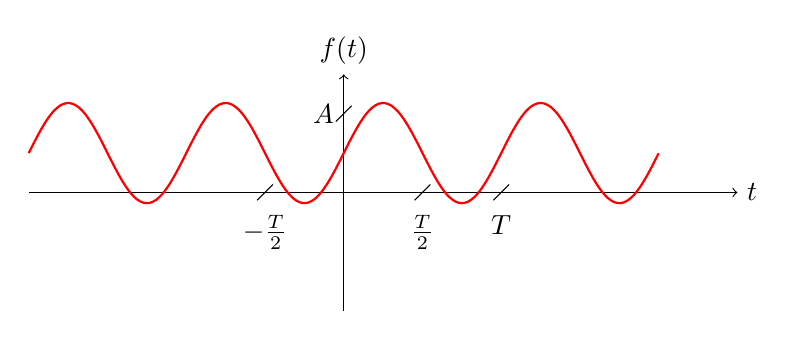
\begin{tikzpicture}
  %\draw (0,0) circle (1in);
  \draw[->] (-4.0,+0.0) -- (+5.0,+0.0) node[right] {$t$};
  \draw[->] (+0.0,-1.5) -- (+0.0,+1.5) node[above] {$f(t)$};
  %\draw[-,red, thick] (-2.5,+0.0) -- (+0.0,+0.0);
  %\draw[-] (-1.0-0.1,-0.1)--(-1.0+0.1,0.1) node[midway, below, outer sep=10pt,align=center] {$-\frac{T}{2}$};
  \draw[-] (-1.0-0.1,-0.1)--(-1.0+0.1,0.1) node[midway, below, outer sep=5pt,align=center] {$-\frac{T}{2}$};
  \draw[-] (+1.0-0.1,-0.1)--(+1.0+0.1,0.1) node[midway, below, outer sep=5pt] {$\frac{T}{2}$};
  \draw[-] (+2.0-0.1,-0.1)--(+2.0+0.1,0.1) node[midway, below, outer sep=5pt] {$T$};
  \draw[-] (-0.1,1.0-0.1)--(+0.1,1.0+0.1) node[midway, left] {$A$};
  
  \draw[scale=1.0,domain=-4:4.0,samples=100,smooth,variable=\x,red,thick] plot ({\x},{0.5+2.0/3.141592*sin(\x*180.0/3.141592*1*3.141592/1.0)});
  \end{tikzpicture}
\end{figure}

\TT{W przypadku sumowania do $k_{max}=3$ otrzymujemy}{A partial approximation of the $f(t)$ signal for $k_{max}=3$ results in:}

\begin{figure}[H]
  \centering
  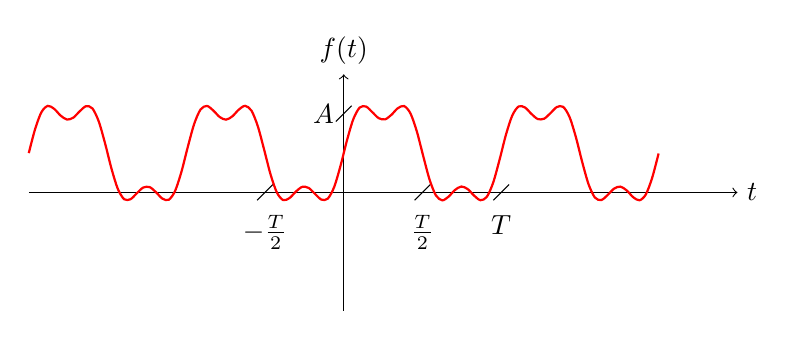
\begin{tikzpicture}
  %\draw (0,0) circle (1in);
  \draw[->] (-4.0,+0.0) -- (+5.0,+0.0) node[right] {$t$};
  \draw[->] (+0.0,-1.5) -- (+0.0,+1.5) node[above] {$f(t)$};
  %\draw[-,red, thick] (-2.5,+0.0) -- (+0.0,+0.0);
  %\draw[-] (-1.0-0.1,-0.1)--(-1.0+0.1,0.1) node[midway, below, outer sep=10pt,align=center] {$-\frac{T}{2}$};
  \draw[-] (-1.0-0.1,-0.1)--(-1.0+0.1,0.1) node[midway, below, outer sep=5pt,align=center] {$-\frac{T}{2}$};
  \draw[-] (+1.0-0.1,-0.1)--(+1.0+0.1,0.1) node[midway, below, outer sep=5pt] {$\frac{T}{2}$};
  \draw[-] (+2.0-0.1,-0.1)--(+2.0+0.1,0.1) node[midway, below, outer sep=5pt] {$T$};
  \draw[-] (-0.1,1.0-0.1)--(+0.1,1.0+0.1) node[midway, left] {$A$};
  
  \draw[scale=1.0,domain=-4:4.0,samples=100,smooth,variable=\x,red,thick] plot ({\x},{0.5+2.0/3.141592*sin(\x*180.0/3.141592*1*3.141592/1.0)+2.0/(3*3.141592)*sin(\x*180.0/3.141592*3*3.141592/1.0)});
  \end{tikzpicture}
\end{figure}

\TT{W przypadku sumowania do $k_{max}=5$ otrzymujemy}{A partial approximation of the $f(t)$ signal for $k_{max}=5$ results in:} 

\begin{figure}[H]
  \centering
  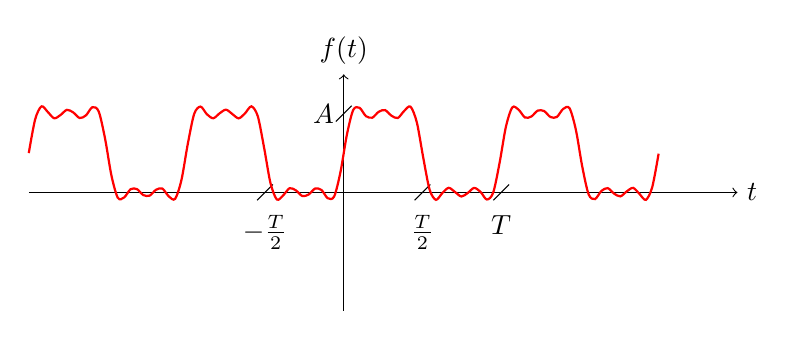
\begin{tikzpicture}
  %\draw (0,0) circle (1in);
  \draw[->] (-4.0,+0.0) -- (+5.0,+0.0) node[right] {$t$};
  \draw[->] (+0.0,-1.5) -- (+0.0,+1.5) node[above] {$f(t)$};
  %\draw[-,red, thick] (-2.5,+0.0) -- (+0.0,+0.0);
  %\draw[-] (-1.0-0.1,-0.1)--(-1.0+0.1,0.1) node[midway, below, outer sep=10pt,align=center] {$-\frac{T}{2}$};
  \draw[-] (-1.0-0.1,-0.1)--(-1.0+0.1,0.1) node[midway, below, outer sep=5pt,align=center] {$-\frac{T}{2}$};
  \draw[-] (+1.0-0.1,-0.1)--(+1.0+0.1,0.1) node[midway, below, outer sep=5pt] {$\frac{T}{2}$};
  \draw[-] (+2.0-0.1,-0.1)--(+2.0+0.1,0.1) node[midway, below, outer sep=5pt] {$T$};
  \draw[-] (-0.1,1.0-0.1)--(+0.1,1.0+0.1) node[midway, left] {$A$};
  
  \draw[scale=1.0,domain=-4:4.0,samples=100,smooth,variable=\x,red,thick] plot ({\x},{0.5+2.0/3.141592*sin(\x*180.0/3.141592*1*3.141592/1.0)+2.0/(3*3.141592)*sin(\x*180.0/3.141592*3*3.141592/1.0)+2.0/(5*3.141592)*sin(\x*180.0/3.141592*5*3.141592/1.0)});
  \end{tikzpicture}
\end{figure}

\TT{W przypadku sumowania do $k_{max}=11$ otrzymujemy}{A partial approximation of the $f(t)$ signal for $k_{max}=11$ results in:}

\begin{figure}[H]
  \centering
  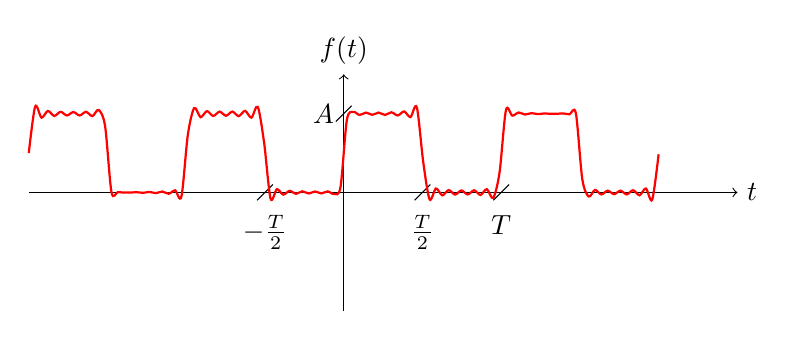
\begin{tikzpicture}
  %\draw (0,0) circle (1in);
  \draw[->] (-4.0,+0.0) -- (+5.0,+0.0) node[right] {$t$};
  \draw[->] (+0.0,-1.5) -- (+0.0,+1.5) node[above] {$f(t)$};
  %\draw[-,red, thick] (-2.5,+0.0) -- (+0.0,+0.0);
  %\draw[-] (-1.0-0.1,-0.1)--(-1.0+0.1,0.1) node[midway, below, outer sep=10pt,align=center] {$-\frac{T}{2}$};
  \draw[-] (-1.0-0.1,-0.1)--(-1.0+0.1,0.1) node[midway, below, outer sep=5pt,align=center] {$-\frac{T}{2}$};
  \draw[-] (+1.0-0.1,-0.1)--(+1.0+0.1,0.1) node[midway, below, outer sep=5pt] {$\frac{T}{2}$};
  \draw[-] (+2.0-0.1,-0.1)--(+2.0+0.1,0.1) node[midway, below, outer sep=5pt] {$T$};
  \draw[-] (-0.1,1.0-0.1)--(+0.1,1.0+0.1) node[midway, left] {$A$};
  
  \draw[scale=1.0,domain=-4:4.0,samples=100,smooth,variable=\x,red,thick] plot ({\x},{0.5+2.0/3.141592*sin(\x*180.0/3.141592*1*3.141592/1.0)+2.0/(3*3.141592)*sin(\x*180.0/3.141592*3*3.141592/1.0)+2.0/(5*3.141592)*sin(\x*180.0/3.141592*5*3.141592/1.0)+2.0/(7*3.141592)*sin(\x*180.0/3.141592*7*3.141592/1.0)+2.0/(9*3.141592)*sin(\x*180.0/3.141592*9*3.141592/1.0)+2.0/(11*3.141592)*sin(\x*180.0/3.141592*11*3.141592/1.0)});
  \end{tikzpicture}
\end{figure}

\TT{W przypadku sumowania do $k_{max}=21$ otrzymujemy}{A partial approximation of the $f(t)$ signal for $k_{max}=21$ results in:}

\begin{figure}[H]
  \centering
  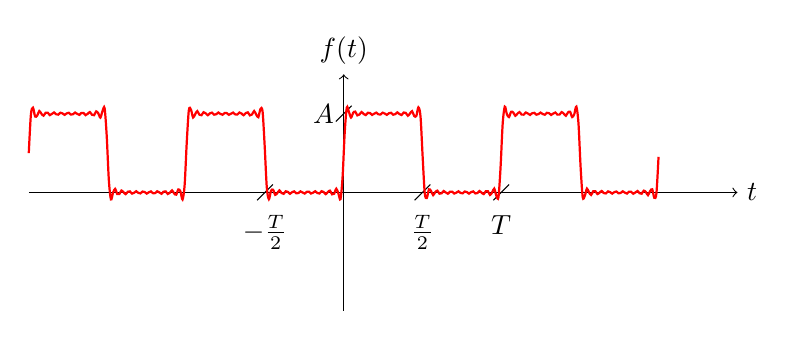
\begin{tikzpicture}
  %\draw (0,0) circle (1in);
  \draw[->] (-4.0,+0.0) -- (+5.0,+0.0) node[right] {$t$};
  \draw[->] (+0.0,-1.5) -- (+0.0,+1.5) node[above] {$f(t)$};
  %\draw[-,red, thick] (-2.5,+0.0) -- (+0.0,+0.0);
  %\draw[-] (-1.0-0.1,-0.1)--(-1.0+0.1,0.1) node[midway, below, outer sep=10pt,align=center] {$-\frac{T}{2}$};
  \draw[-] (-1.0-0.1,-0.1)--(-1.0+0.1,0.1) node[midway, below, outer sep=5pt,align=center] {$-\frac{T}{2}$};
  \draw[-] (+1.0-0.1,-0.1)--(+1.0+0.1,0.1) node[midway, below, outer sep=5pt] {$\frac{T}{2}$};
  \draw[-] (+2.0-0.1,-0.1)--(+2.0+0.1,0.1) node[midway, below, outer sep=5pt] {$T$};
  \draw[-] (-0.1,1.0-0.1)--(+0.1,1.0+0.1) node[midway, left] {$A$};
  
  \draw[scale=1.0,domain=-4:4.0,samples=300,smooth,variable=\x,red,thick] plot ({\x},{0.5+2.0/3.141592*sin(\x*180.0/3.141592*1*3.141592/1.0)+2.0/(3*3.141592)*sin(\x*180.0/3.141592*3*3.141592/1.0)+2.0/(5*3.141592)*sin(\x*180.0/3.141592*5*3.141592/1.0)+2.0/(7*3.141592)*sin(\x*180.0/3.141592*7*3.141592/1.0)+2.0/(9*3.141592)*sin(\x*180.0/3.141592*9*3.141592/1.0)+2.0/(11*3.141592)*sin(\x*180.0/3.141592*11*3.141592/1.0)+2.0/(13*3.141592)*sin(\x*180.0/3.141592*13*3.141592/1.0)+2.0/(15*3.141592)*sin(\x*180.0/3.141592*15*3.141592/1.0)+2.0/(17*3.141592)*sin(\x*180.0/3.141592*17*3.141592/1.0)+2.0/(19*3.141592)*sin(\x*180.0/3.141592*19*3.141592/1.0)+2.0/(21*3.141592)*sin(\x*180.0/3.141592*21*3.141592/1.0)});
  \end{tikzpicture}
\end{figure}

\TT{W granicy sumowania do $k_{max}=\infty$ otrzymujemy oryginalny sygnał.}{Approximation of the $f(t)$ signal for $k_{max}=\infty$ results in oryginal signal.}

\end{task}